% Options for packages loaded elsewhere
\PassOptionsToPackage{unicode}{hyperref}
\PassOptionsToPackage{hyphens}{url}
%
\documentclass[
  x11names]{article}
\usepackage{amsmath,amssymb}
\usepackage{lmodern}
\usepackage{iftex}
\ifPDFTeX
  \usepackage[T1]{fontenc}
  \usepackage[utf8]{inputenc}
  \usepackage{textcomp} % provide euro and other symbols
\else % if luatex or xetex
  \usepackage{unicode-math}
  \defaultfontfeatures{Scale=MatchLowercase}
  \defaultfontfeatures[\rmfamily]{Ligatures=TeX,Scale=1}
\fi
% Use upquote if available, for straight quotes in verbatim environments
\IfFileExists{upquote.sty}{\usepackage{upquote}}{}
\IfFileExists{microtype.sty}{% use microtype if available
  \usepackage[]{microtype}
  \UseMicrotypeSet[protrusion]{basicmath} % disable protrusion for tt fonts
}{}
\makeatletter
\@ifundefined{KOMAClassName}{% if non-KOMA class
  \IfFileExists{parskip.sty}{%
    \usepackage{parskip}
  }{% else
    \setlength{\parindent}{0pt}
    \setlength{\parskip}{6pt plus 2pt minus 1pt}}
}{% if KOMA class
  \KOMAoptions{parskip=half}}
\makeatother
\usepackage{xcolor}
\usepackage[margin=1in]{geometry}
\usepackage{graphicx}
\makeatletter
\def\maxwidth{\ifdim\Gin@nat@width>\linewidth\linewidth\else\Gin@nat@width\fi}
\def\maxheight{\ifdim\Gin@nat@height>\textheight\textheight\else\Gin@nat@height\fi}
\makeatother
% Scale images if necessary, so that they will not overflow the page
% margins by default, and it is still possible to overwrite the defaults
% using explicit options in \includegraphics[width, height, ...]{}
\setkeys{Gin}{width=\maxwidth,height=\maxheight,keepaspectratio}
% Set default figure placement to htbp
\makeatletter
\def\fps@figure{htbp}
\makeatother
\setlength{\emergencystretch}{3em} % prevent overfull lines
\providecommand{\tightlist}{%
  \setlength{\itemsep}{0pt}\setlength{\parskip}{0pt}}
\setcounter{secnumdepth}{-\maxdimen} % remove section numbering
\usepackage{fontspec} \usepackage{titling} \pretitle{\begin{center} \LARGE \vspace{-3.3cm} 
\includegraphics[width=\linewidth]{images/Base_info/logo.png}\\} \posttitle{\end{center}} \usepackage{framed} \usepackage{float} \usepackage{fancyhdr} \usepackage{ragged2e} \usepackage{caption} \usepackage{colortbl} \usepackage[export]{adjustbox} \usepackage{wrapfig} \captionsetup[figure]{labelformat=empty} \arrayrulecolor{white} \pagestyle{fancy} \fancyhead[L,C]{} \fancypagestyle{plain}{\pagestyle{fancy}} \PassOptionsToPackage{dvipsnames,svgnames*,x11names*}{xcolor} \definecolor{ceil}{rgb}{0.57, 0.63, 0.81}
\usepackage{booktabs}
\usepackage{longtable}
\usepackage{array}
\usepackage{multirow}
\usepackage{wrapfig}
\usepackage{float}
\usepackage{colortbl}
\usepackage{pdflscape}
\usepackage{tabu}
\usepackage{threeparttable}
\usepackage{threeparttablex}
\usepackage[normalem]{ulem}
\usepackage{makecell}
\usepackage{xcolor}
\ifLuaTeX
  \usepackage{selnolig}  % disable illegal ligatures
\fi
\IfFileExists{bookmark.sty}{\usepackage{bookmark}}{\usepackage{hyperref}}
\IfFileExists{xurl.sty}{\usepackage{xurl}}{} % add URL line breaks if available
\urlstyle{same} % disable monospaced font for URLs
\hypersetup{
  pdftitle={~},
  hidelinks,
  pdfcreator={LaTeX via pandoc}}

\title{~}
\author{}
\date{\vspace{-2.5em}}

\begin{document}
\maketitle

\renewenvironment{framed}[1][\hsize]
  {\MakeFramed{\hsize#1\advance\hsize-\width \FrameRestore}}%
  {\endMakeFramed}

\setmainfont{Arial}
\setsansfont{Arial}
\setmonofont{Arial}

\newcommand\invisiblesection[1]{%
  \refstepcounter{section}%
  \addcontentsline{toc}{section}{\protect\numberline{\thesection}#1}%
  \sectionmark{#1}}

\fancyhead[R]{\textbf{http://doi.org/10.31687/SaremLR.19.202}}

%
  \refstepcounter{section}%
  \addcontentsline{toc}{section}{\protect\numberline{\thesection}GENERALIDADES}%
  \sectionmark{GENERALIDADES}

\vspace{-3cm}

\begin{minipage}{0.75\textwidth}
\vspace{0.15cm}
{\fontsize{18}{22}\selectfont\textit{Parachoerus wagneri}}

\vspace{0.3cm}
{\fontsize{30}{36}\selectfont\textbf{Pecarí quimilero}}
\end{minipage}
\hspace{0.05\textwidth}
\begin{minipage}{0.2\textwidth}

\includegraphics[width=\textwidth]{images/en.png}\\
\end{minipage}

\normalsize

\begin{figure}[H]

{\centering \includegraphics[width=0.95\linewidth]{photos//Cetaartiodactyla/202_Parachoerus-wagneri_1_Yamil-Di-Blanco} 

}

\caption{Foto: Yamil Di Blanco}\label{fig:photo}
\end{figure}

\vspace{-1cm}

\begin{center}\rule{0.5\linewidth}{0.5pt}\end{center}

\justifying

\textbf{Cita sugerida:} Camino, Micaela; Torres, Ricardo M.. (2019).
\emph{Parachoerus wagneri}. En: SAyDS--SAREM (eds.) Categorización 2019
de los mamíferos de Argentina según su riesgo de extinción. Lista Roja
de los mamíferos de Argentina.
\url{http://doi.org/10.31687/SaremLR.19.202}

\begin{center}\rule{0.5\linewidth}{0.5pt}\end{center}

\newpage

\vspace{-0.4cm}

%
  \refstepcounter{section}%
  \addcontentsline{toc}{section}{\protect\numberline{\thesection}OTRAS FOTOGRAFÍAS}%
  \sectionmark{OTRAS FOTOGRAFÍAS}
\begin{table}[H]
\centering
\begin{tabular}[t]{>{\raggedright\arraybackslash}m{16cm}>{}m{16cm}}
\toprule
\cellcolor{ceil}{\textcolor{white}{\textbf{\rule{0pt}{14pt}OTRAS FOTOGRAFÍAS}}}\\
\bottomrule
\end{tabular}
\end{table}\vspace{-0.5cm}

\begin{figure}[H]\centering\includegraphics[width=0.850\textwidth]{photos//Cetaartiodactyla/202_Parachoerus-wagneri_2_Francisco-Erize_0.jpg}\caption{Foto: Francisco Erize}\end{figure}

\vspace{-0.3cm}\begin{figure}[H]\centering\includegraphics[width=0.850\textwidth]{photos//Cetaartiodactyla/202_Parachoerus-wagneri_3_Jose-Cartes.jpg}\caption{Foto: Jose Cartes}\end{figure}

\vspace{-0.3cm}

\newpage

\vspace{-0.4cm}

%
  \refstepcounter{section}%
  \addcontentsline{toc}{section}{\protect\numberline{\thesection}ÁREA DE DISTRIBUCIÓN ACTUAL}%
  \sectionmark{ÁREA DE DISTRIBUCIÓN ACTUAL}
\begin{table}[H]
\centering
\begin{tabular}[t]{>{\raggedright\arraybackslash}m{16cm}>{}m{16cm}}
\toprule
\cellcolor{ceil}{\textcolor{white}{\textbf{\rule{0pt}{14pt}ÁREA DE DISTRIBUCIÓN ACTUAL}}}\\
\bottomrule
\end{tabular}
\end{table}

\vspace{-0.4cm}

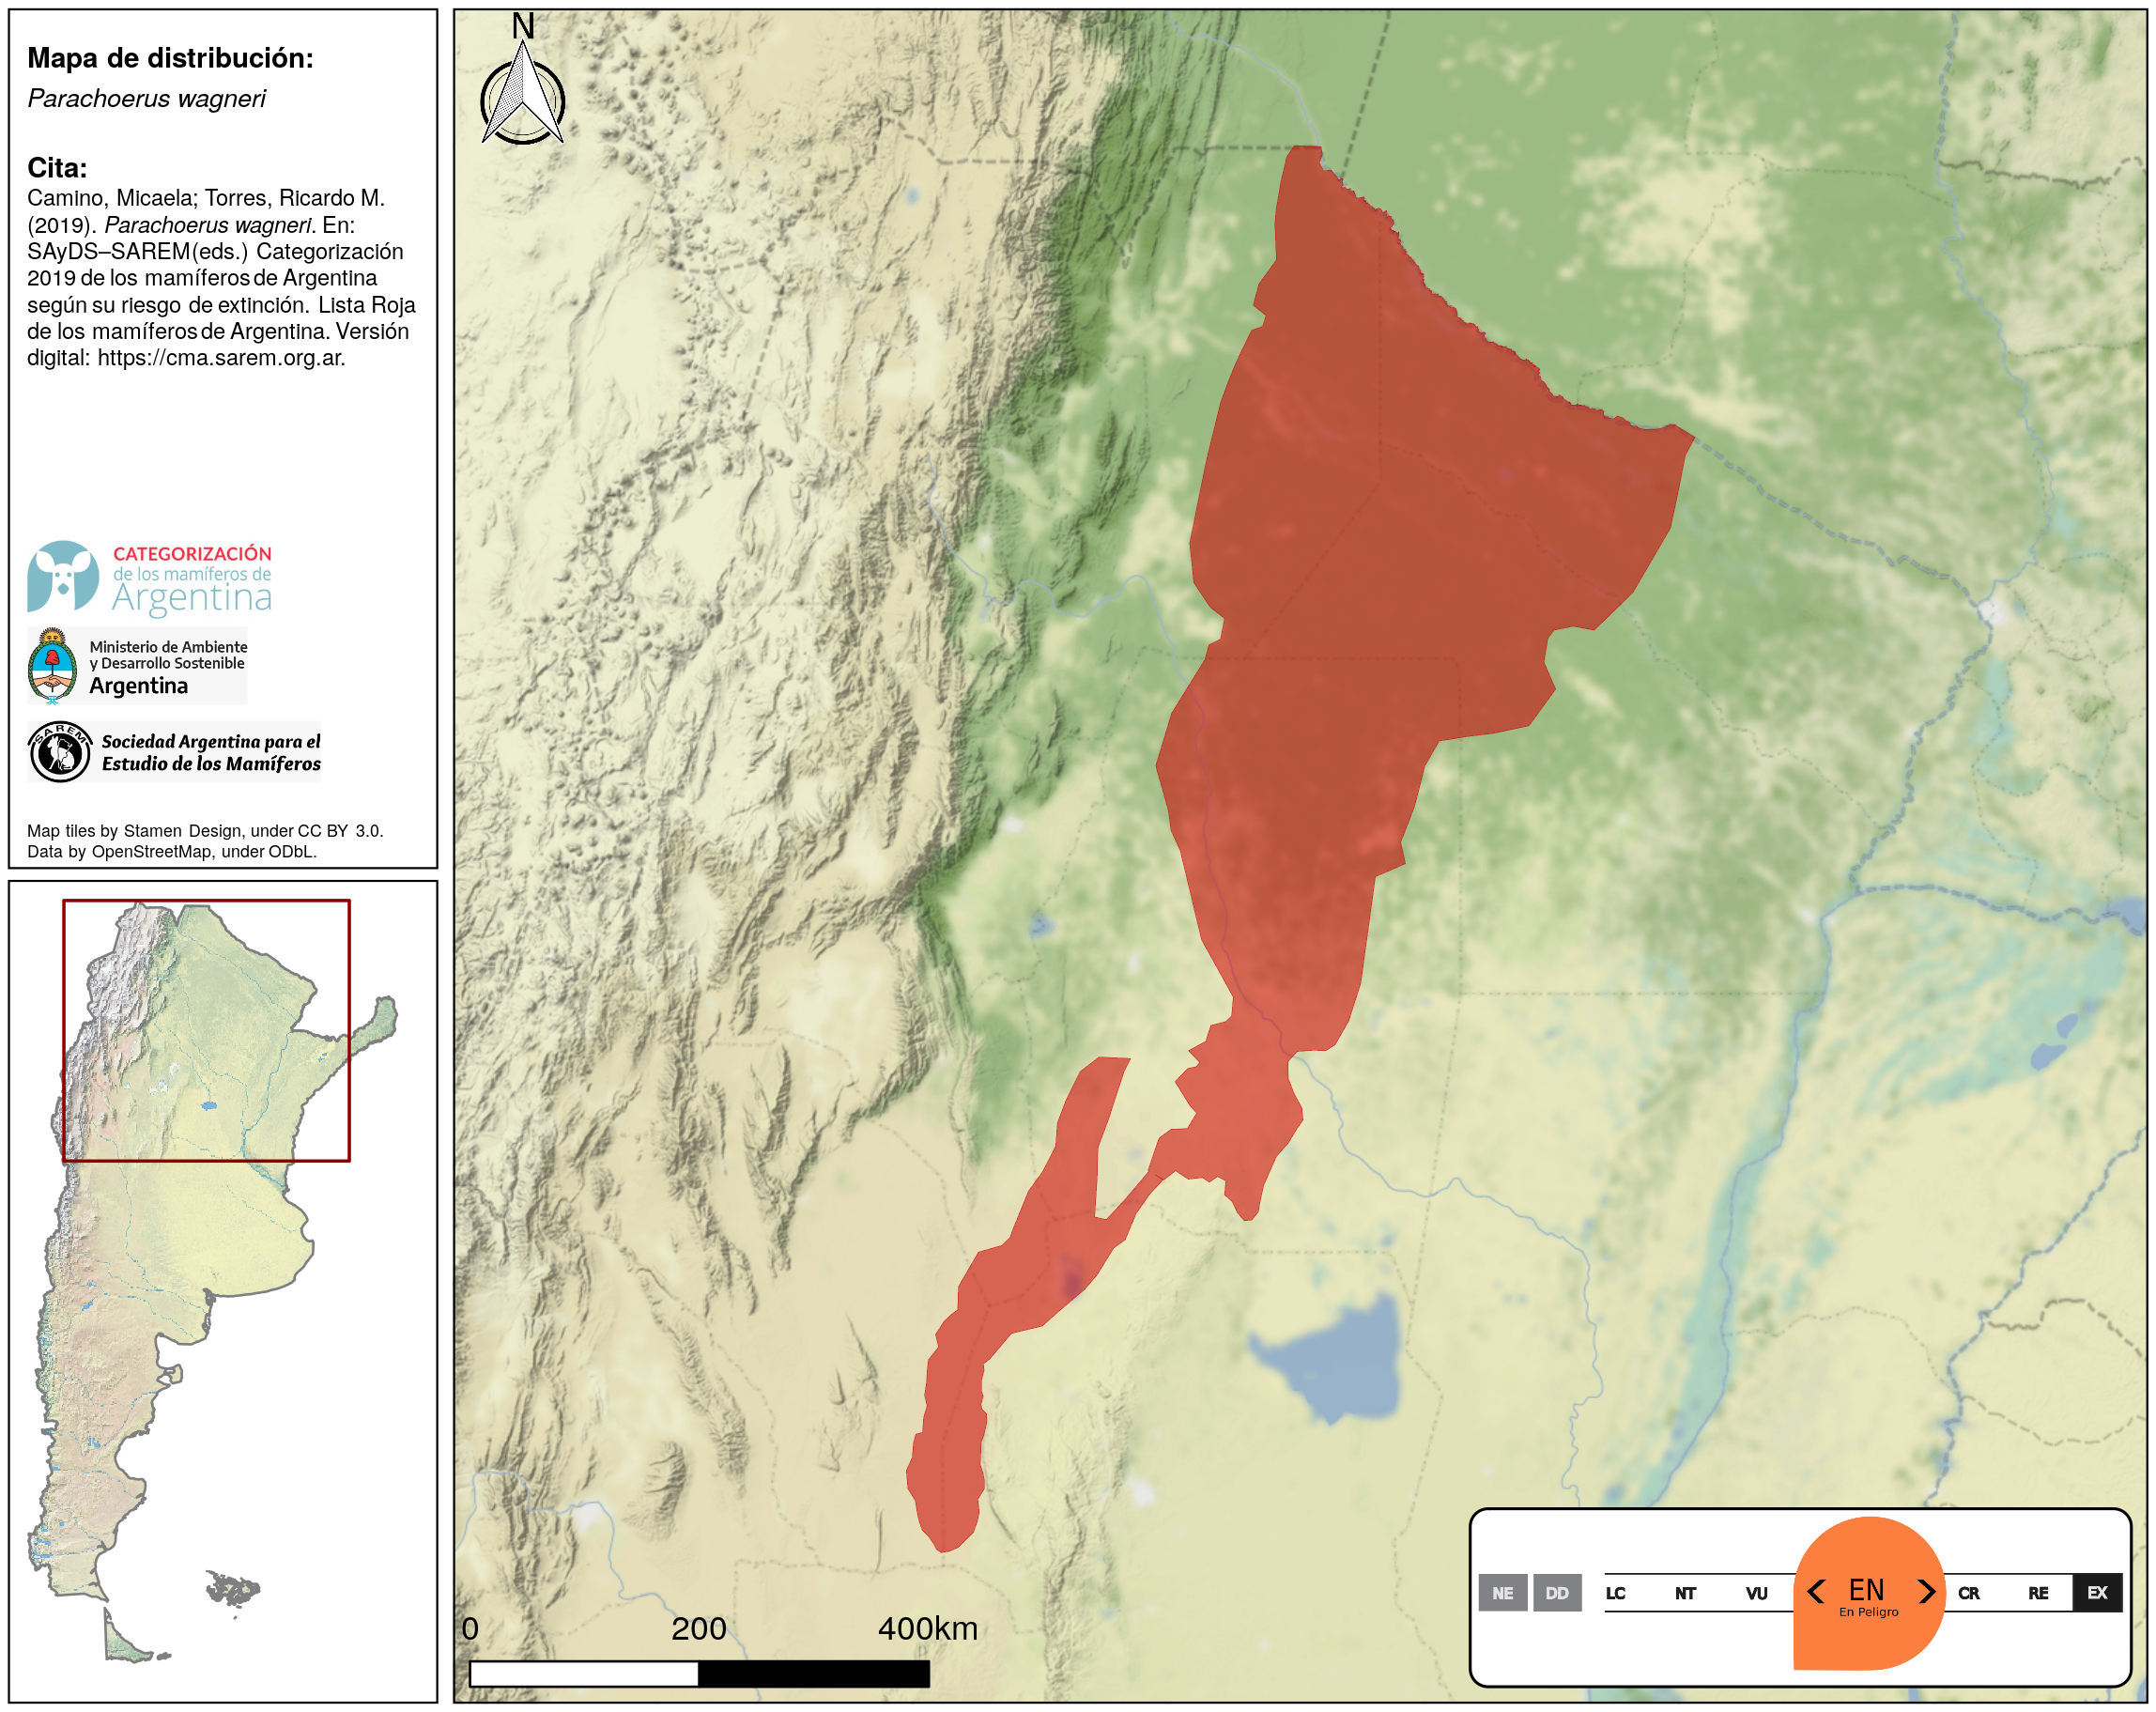
\includegraphics[width=1\linewidth]{maps/Cetartiodactyla/Parachoerus_wagneri}

%
  \refstepcounter{section}%
  \addcontentsline{toc}{section}{\protect\numberline{\thesection}CATEGORÍAS DE CONSERVACIÓN}%
  \sectionmark{CATEGORÍAS DE CONSERVACIÓN}
\begin{table}[H]
\centering
\begin{tabular}[t]{>{\raggedright\arraybackslash}m{16cm}>{}m{16cm}}
\toprule
\cellcolor{ceil}{\textcolor{white}{\textbf{\rule{0pt}{14pt}CATEGORÍAS DE CONSERVACIÓN}}}\\
\bottomrule
\end{tabular}
\end{table}

\vspace{-0.4cm}

\begin{tabu} to \linewidth {>{\raggedright}X>{\raggedright}X}
\toprule
\textbf{Categoría Nacional de Conservación 2019} & \textbf{Criterios y subcriterios}\\
\midrule
\cellcolor{gray!6}{EN (En Peligro)} & \cellcolor{gray!6}{A3cd}\\
\bottomrule
\end{tabu}

\textbf{Justificación de la categorización}

El pecarí quimilero es un especialista de hábitat, habitando casi
exclusivamente bosques nativos. La especie es endémica del Gran Chaco,
particularmente del Chaco Seco, y por lo tanto se lo encuentra casi
exclusivamente en bosques chaqueños primarios o, en menor medida en,
secundarios. En los últimos 30 años un 20\% de los bosques chaqueños ha
sido reemplazado por cultivos y pasturas (Baumann et al.~2017) y la
especie es activamente cazada en toda su área de distribución. Por lo
tanto, se sospecha que, de continuar la actual tendencia de
deforestación y extracción de individuos, la especie experimentará una
reducción de más del 50\% de su población en las próximas 3 generaciones
(12 años) por reducción de AOO y EOO, degradación del hábitat y
sobre-cacería. Por lo expuesto esta especie es categorizada como En
Peligro (EN) siguiendo el criterio A3cd.

\textbf{Categoría Res. SAyDS 1030/04}

EP (En Peligro de Extinción)

\textbf{Categorías nacionales de conservación previas (SAREM)}

\begin{tabu} to \linewidth {>{}l>{\raggedright}X>{\raggedright}X}
\toprule
\textbf{\cellcolor{gray!6}{2012}} & \cellcolor{gray!6}{EN (En Peligro)} & \cellcolor{gray!6}{A3cd+4cd}\\
\bottomrule
\end{tabu}

\begin{tabu} to \linewidth {>{}l>{\raggedright}X>{\raggedright}X}
\toprule
\textbf{\cellcolor{gray!6}{2000}} & \cellcolor{gray!6}{VU (Vulnerable)} & \cellcolor{gray!6}{B1}\\
\bottomrule
\end{tabu}

\begin{tabu} to \linewidth {>{}l>{\raggedright}X>{\raggedright}X}
\toprule
\textbf{\cellcolor{gray!6}{1997}} & \cellcolor{gray!6}{VU (Vulnerable)} & \cellcolor{gray!6}{B1}\\
\bottomrule
\end{tabu}

\begin{tabu} to \linewidth {>{}l>{\raggedright}X}
\toprule
\textbf{\cellcolor{gray!6}{Homologación categoría 1997}} & \cellcolor{gray!6}{VU (Vulnerable)}\\
\bottomrule
\end{tabu}

\textbf{Categorías de conservación actuales en países vecinos}

\begin{tabu} to \linewidth {>{\raggedright}X>{\raggedright}X>{\raggedright}X>{\raggedright}X}
\toprule
\textbf{País} & \textbf{Categoría} & \textbf{Año} & \textbf{Cita}\\
\arrayrulecolor{white}
\midrule
\cellcolor{gray!6}{Bolivia} & \cellcolor{gray!6}{EN (En Peligro)} & \cellcolor{gray!6}{2009} & \cellcolor{gray!6}{Tarifa \&amp; Aguirre (2009)}\\
\bottomrule
\end{tabu}
\begin{tabu} to \linewidth {>{\raggedright}X>{\raggedright}X>{\raggedright}X>{\raggedright}X}
\toprule
\textbf{País} & \textbf{Categoría} & \textbf{Año} & \textbf{Cita}\\
\arrayrulecolor{white}
\midrule
\cellcolor{gray!6}{Paraguay} & \cellcolor{gray!6}{EN (En Peligro)} & \cellcolor{gray!6}{2017} & \cellcolor{gray!6}{Cartes et al. (2017)}\\
\bottomrule
\end{tabu}

\textbf{Evaluación global UICN}

\begin{tabu} to \linewidth {>{\raggedright}X>{\raggedright}X>{\raggedright}X}
\toprule
\textbf{Año de evaluación} & \textbf{Categoría} & \textbf{Criterios y subcriterios}\\
\arrayrulecolor{white}
\midrule
\cellcolor{gray!6}{2015} & \cellcolor{gray!6}{EN (En Peligro)} & \cellcolor{gray!6}{A3 cd + 4 cd}\\
\bottomrule
\end{tabu}

\arrayrulecolor{white}

%
  \refstepcounter{section}%
  \addcontentsline{toc}{section}{\protect\numberline{\thesection}TAXONOMÍA Y NOMENCLATURA}%
  \sectionmark{TAXONOMÍA Y NOMENCLATURA}
\begin{table}[H]
\centering
\begin{tabular}[t]{>{\raggedright\arraybackslash}m{16cm}>{}m{16cm}}
\toprule
\cellcolor{ceil}{\textcolor{white}{\textbf{\rule{0pt}{14pt}TAXONOMÍA Y NOMENCLATURA}}}\\
\bottomrule
\end{tabular}
\end{table}

\vspace{-0.4cm}

\begin{tabu} to \linewidth {>{\raggedright\arraybackslash}p{6cm}>{\raggedright\arraybackslash}p{1cm}>{\raggedright}X}
\toprule
\textbf{\cellcolor{gray!6}{Orden}} & \cellcolor{gray!6}{} & \cellcolor{gray!6}{Cetartiodactyla}\\
\bottomrule
\end{tabu} \vspace{0.3cm}
\begin{tabu} to \linewidth {>{\raggedright\arraybackslash}p{6cm}>{\raggedright\arraybackslash}p{1cm}>{\raggedright}X}
\toprule
\textbf{\cellcolor{gray!6}{Familia}} & \cellcolor{gray!6}{} & \cellcolor{gray!6}{Tayassuidae}\\
\bottomrule
\end{tabu} \vspace{0.3cm}
\begin{tabu} to \linewidth {>{\raggedright\arraybackslash}p{6cm}>{\raggedright\arraybackslash}p{1cm}>{\raggedright}X}
\toprule
\textbf{\cellcolor{gray!6}{Nombre científico}} & \cellcolor{gray!6}{} & \cellcolor{gray!6}{\textit{Parachoerus wagneri} (Rusconi, 1930)}\\
\bottomrule
\end{tabu} \vspace{0.3cm}
\begin{tabu} to \linewidth {>{\raggedright\arraybackslash}p{6cm}>{\raggedright\arraybackslash}p{1cm}>{\raggedright}X}
\toprule
\textbf{\cellcolor{gray!6}{Nombre común}} & \cellcolor{gray!6}{} & \cellcolor{gray!6}{Pecarí quimilero}\\
\bottomrule
\end{tabu} \vspace{0.3cm}
\begin{tabu} to \linewidth {>{\raggedright\arraybackslash}p{6cm}>{\raggedright\arraybackslash}p{1cm}>{\raggedright}X}
\toprule
\textbf{\cellcolor{gray!6}{Nombres comunes locales}} & \cellcolor{gray!6}{} & \cellcolor{gray!6}{Quimilero}\\
\textbf{} &  & Chancho quimilero\\
\textbf{\cellcolor{gray!6}{}} & \cellcolor{gray!6}{} & \cellcolor{gray!6}{Chancho moro}\\
\textbf{} &  & Collarejo\\
\bottomrule
\end{tabu} \vspace{0.3cm}
\begin{tabu} to \linewidth {>{\raggedright\arraybackslash}p{6cm}>{\raggedright\arraybackslash}p{1cm}>{\raggedright}X}
\toprule
\textbf{\cellcolor{gray!6}{Nombres comunes en inglés}} & \cellcolor{gray!6}{} & \cellcolor{gray!6}{Chacoan Peccary}\\
\bottomrule
\end{tabu} \vspace{0.3cm}

\textbf{Comentarios taxonómicos}

La relación filogenética entre las diferentes especies de pecaríes,
vivas y extintas, no es clara (Parisi-Dutra et al.~2017). Wright (1998)
diferenció las subfamilias morfofiléticas Hesperhyinae y Tayassuinae y
colocó a la especie dentro del género Catagonus, hermana del género
Pecari. Góngora \& Moran (2005) mantuvieron la existencia del género
Catagonus y consideraron que el grupo también era hermano del género
Tayassu. Parisi-Dutra et al.~(2017) analizaron la filogenia de pecaríes
y concluyeron que el género Catagonus es un grupo parafilético en el
cual no se encontraría esta especie, que ubican en el género
\textit{Parachoerus}. Sinónimo: Catagonus wagneri~Rusconi, 1930

\arrayrulecolor{white}

%
  \refstepcounter{section}%
  \addcontentsline{toc}{section}{\protect\numberline{\thesection}INFORMACIÓN RELEVANTE PARA LA EVALUACIÓN}%
  \sectionmark{INFORMACIÓN RELEVANTE PARA LA EVALUACIÓN}
\begin{table}[H]
\centering
\begin{tabular}[t]{>{\raggedright\arraybackslash}m{16cm}>{}m{16cm}}
\toprule
\cellcolor{ceil}{\textcolor{white}{\textbf{\rule{0pt}{14pt}INFORMACIÓN RELEVANTE PARA LA EVALUACIÓN}}}\\
\bottomrule
\end{tabular}
\end{table}

\vspace{-0.4cm}

%
  \refstepcounter{section}%
  \addcontentsline{toc}{section}{\protect\numberline{\thesection}RANGO GEOGRÁFICO, OCURRENCIA Y ABUNDANCIA}%
  \sectionmark{RANGO GEOGRÁFICO, OCURRENCIA Y ABUNDANCIA}
\begin{table}[H]
\centering
\begin{tabular}[t]{>{\raggedright\arraybackslash}m{16cm}>{}m{16cm}}
\toprule
\cellcolor{ceil}{\textcolor{white}{\textbf{\rule{0pt}{14pt}RANGO GEOGRÁFICO, OCURRENCIA Y ABUNDANCIA}}}\\
\bottomrule
\end{tabular}
\end{table}

\vspace{-0.4cm}

\textbf{Presencia en el territorio nacional:} residente

\textbf{Comentarios sobre la distribución actual e histórica}

La especie es endémica de la ecorregión chaqueña (Sowls 1997). Existen
registros fósiles en otras áreas que habrían tenido características
ambientales cálidas y secas, i.e.~Uruguay en Pleistoceno (Gasparini et
al.~2013). La distribución actual no es completamente conocida, lo cual
quedó demostrado hace poco cuando Torres et al.~(2017) detectaron la
presencia de P. wagneri a más de 650 km al sur del límite de su
distribución conocida. Posteriormente, nuevos hallazgos lo confirman
para el sur de Santiago del Estero, oeste de Córdoba (Torres et
al.~2018) y este de La Rioja, concordando con lo previamente explorado
mediante un modelo de distribución (Altrichter et al.~2016), según el
cual se estimó que una superficie de 497.577 km2 en el Gran Chaco
(correspondiente a un 46,24\% del mismo) está constituida de hábitats
óptimos para la especie. Todos los hallazgos realizados hasta el momento
en Córdoba y La Rioja se concentran en el área de influencia del Parque
Nacional Traslasierra, en donde su presencia ya ha sido ratificada
(Torres et al.~2017) y vuelta a confirmar mediante el uso de cámaras
trampa (en el marco de un proyecto que evalúa la defaunación de la
región; IDEA-CONICET). La especie también ha sido buscada en las áreas
que conectan el sur de Santiago del Estero con el oeste de Córdoba y
este de La Rioja, a través de monitoreo con cámaras-trampa, y mediante
entrevistas con pobladores locales. Sin embargo, hasta el momento la
especie no ha sido hallada en estas áreas intermedias, a pesar de que en
algunos sitios los entrevistados la reconocieron sin lugar a dudas. La
información recabada hasta el momento sugiere que la población del oeste
de Córdoba y este de La Rioja se encuentra en riesgo de aislamiento o ya
aislada del resto, siendo las causas más probables la sobrecaza y la
degradación del hábitat en dichas áreas intermedias, aunque son
necesarios más estudios que confirmen o refuten esta afirmación. Dado
que los requerimientos de hábitat de la especie son restringidos, la
acelerada pérdida de hábitat asociada a la conversión de bosques a
cultivos y pasturas estaría reduciendo aceleradamente la distribución de
la especie. La tasa de deforestación en el Chaco es una de las más
aceleradas del mundo (Baumann et al.~2017).

\begin{tabu} to \linewidth {>{\raggedright\arraybackslash}p{8cm}>{\raggedright\arraybackslash}p{0.5cm}>{\raggedright}X}
\toprule
\textbf{\cellcolor{gray!6}{Presencia confirmada por provincia:}} & \cellcolor{gray!6}{} & \cellcolor{gray!6}{Chaco}\\
\textbf{} &  & Córdoba\\
\textbf{\cellcolor{gray!6}{}} & \cellcolor{gray!6}{} & \cellcolor{gray!6}{Formosa}\\
\textbf{} &  & La Rioja\\
\textbf{\cellcolor{gray!6}{}} & \cellcolor{gray!6}{} & \cellcolor{gray!6}{Salta}\\
\textbf{} &  & Santiago del Estero\\
\bottomrule
\end{tabu}

\begin{tabu} to \linewidth {>{\raggedright\arraybackslash}p{8cm}>{\raggedright\arraybackslash}p{0.5cm}>{\raggedright}X}
\toprule
\textbf{\cellcolor{gray!6}{Presencia en ecorregiones de Argentina:}} & \cellcolor{gray!6}{} & \cellcolor{gray!6}{Chaco Seco}\\
\textbf{} &  & Chaco Húmedo\\
\bottomrule
\end{tabu}

\begin{tabu} to \linewidth {>{\raggedright\arraybackslash}p{8cm}>{\raggedright\arraybackslash}p{0.5cm}>{\raggedright}X}
\toprule
\textbf{\cellcolor{gray!6}{Presencia en ecorregiones globales terrestres:}} & \cellcolor{gray!6}{} & \cellcolor{gray!6}{ID569 – Chaco Seco}\\
\textbf{} &  & ID571 – Chaco Húmedo\\
\bottomrule
\end{tabu}

\begin{tabu} to \linewidth {>{\raggedright}X>{\raggedright}X>{\raggedright}X}
\toprule
\textbf{Patrón de distribución} & \textbf{Cantidad de localidades} & \textbf{Rango altitudinal}\\
\midrule
\cellcolor{gray!6}{continuo} & \cellcolor{gray!6}{NA} & \cellcolor{gray!6}{0-500 msnm}\\
\bottomrule
\end{tabu}

\begin{tabu} to \linewidth {>{}l>{\raggedright}X}
\toprule
\textbf{\cellcolor{gray!6}{Endemismo}} & \cellcolor{gray!6}{especie endémica ecorregional}\\
\bottomrule
\end{tabu}

\begin{tabu} to \linewidth {>{}l>{\raggedright}X}
\toprule
\textbf{\cellcolor{gray!6}{Abundancia relativa estimada en su área de ocupación}} & \cellcolor{gray!6}{escasa}\\
\bottomrule
\end{tabu}

\textbf{Comentarios sobre la abundancia, densidad o probabilidad de
ocupación de la especie}

En un área de 54.000 km2 Camino (2016) estimó que la probabilidad de que
P. wagneri ocupe un área de 36 km2 era de 0,86. Los datos fueron
colectados entre 2011 y 2013 en porciones de las Provincias de Chaco,
Formosa y Salta que conservaban en ese momento grandes extensiones
continuas de bosques nativos y otras coberturas naturales. La presencia
de cactáceas, la diversidad de coberturas vegetales y la disponibilidad
de bosques secundarios se asocia positivamente con la probabilidad de
que un territorio esté ocupado por la especie (Camino 2016). La
presencia humana se relaciona negativamente con esta probabilidad,
excepto por áreas cercanas a rutas, que tendrían una probabilidad mayor
a la esperada por el azar de tener la especie (Camino 2016). En el área
del Parque Nacional Defensores del Chaco y en sus alrededores, en
Paraguay, la probabilidad de ocupación fue de 0,37 (Saldivar 2014). Aquí
también se vió una asociación positiva entre P. wagneri y las rutas
asfaltadas. Estudios de ocupación en matrices de producción intensiva
encontraron la presencia de la especie en cortinas boscosas
(Núñez-Regueiro et al.~2015). Desconocemos el tiempo de retraso de las
poblaciones de P. wagneri a la pérdida de hábitat.

\textbf{¿Existen actualmente programas de monitoreo?:} sí

En una superficie de 2400 km2 del Chaco Seco, entre 2011-2017, existió
un programa de monitoreo participativo de base local (Camino 2014;
Camino et al.~2017). Luego del hallazgo de la especie en dos localidades
en el oeste de Córdoba, a más de 650 km del área de distribución
conocida (Torres et al.~2017), en la actualidad se está llevando a cabo
un relevamiento de la presencia de la especie en áreas que no habían
sido prospectadas a tal fin
(\url{https://www.speciesconservation.org/case-studies-projects/chacoan-peccary/13628}),
confirmándose la presencia de la especie en el oeste de Córdoba, y
además en el sur de Santiago del Estero (Torres et al.~2018), y este de
La Rioja.

\arrayrulecolor{white}

%
  \refstepcounter{section}%
  \addcontentsline{toc}{section}{\protect\numberline{\thesection}DATOS MORFOMÉTRICOS}%
  \sectionmark{DATOS MORFOMÉTRICOS}
\begin{table}[H]
\centering
\begin{tabular}[t]{>{\raggedright\arraybackslash}m{16cm}>{}m{16cm}}
\toprule
\cellcolor{ceil}{\textcolor{white}{\textbf{\rule{0pt}{14pt}DATOS MORFOMÉTRICOS}}}\\
\bottomrule
\end{tabular}
\end{table}

\vspace{-0.4cm}

\begin{tabu} to \linewidth {>{\raggedright}X}
\toprule
\textbf{Peso}\\
\midrule
\cellcolor{gray!6}{30-40 kg}\\
\bottomrule
\end{tabu}

\arrayrulecolor{white}

%
  \refstepcounter{section}%
  \addcontentsline{toc}{section}{\protect\numberline{\thesection}RASGOS ETO-ECOLÓGICOS}%
  \sectionmark{RASGOS ETO-ECOLÓGICOS}
\begin{table}[H]
\centering
\begin{tabular}[t]{>{\raggedright\arraybackslash}m{16cm}>{}m{16cm}}
\toprule
\cellcolor{ceil}{\textcolor{white}{\textbf{\rule{0pt}{14pt}RASGOS ETO-ECOLÓGICOS}}}\\
\bottomrule
\end{tabular}
\end{table}

\vspace{-0.4cm}

\textbf{Hábitos:} terrestres

\textbf{Hábitos especializados:} cursorial

\textbf{Otro hábito especializado: comentarios}

NA

\textbf{Dieta:} omnívoro

\textbf{Dieta especializada:} NA

\textbf{Aspectos reproductivos}

Parachoerus wagneri alcanza la madurez sexual a los 2 años. Sowls (1997)
indicó que la reproducción ocurre entre entre abril y mayo, la gestación
dura 150-184 días, los nacimientos son entre septiembre y diciembre y
nacen entre 1 y 4 crías. Los pobladores del Chaco Seco argentino indican
que si bien la mayor parte de los nacimientos ocurren en esa época, en
realidad P. wagneri puede tener crías a lo largo de todo el año y que
normalmente nace un solo individuo por madre (Camino M., obs. pers.).
Las crías pueden seguir a la piara a la semana de nacidas.

\textbf{Patrón de actividad:} diurno, crepuscular

\textbf{Gregariedad:} especie grupal

En Córdoba y La Rioja solo se observan grupos de entre 1 y 3 individuos

\textbf{Área de acción}

Es una especie territorial y su área de acción en el Chaco Paraguayo fue
estimada en 11-15 km2 (Taber et al.~1993).

%
  \refstepcounter{section}%
  \addcontentsline{toc}{section}{\protect\numberline{\thesection}CONSERVACIÓN E INVESTIGACIÓN}%
  \sectionmark{CONSERVACIÓN E INVESTIGACIÓN}
\begin{table}[H]
\centering
\begin{tabular}[t]{>{\raggedright\arraybackslash}m{16cm}>{}m{16cm}}
\toprule
\cellcolor{ceil}{\textcolor{white}{\textbf{\rule{0pt}{14pt}CONSERVACIÓN E INVESTIGACIÓN}}}\\
\bottomrule
\end{tabular}
\end{table}

\vspace{-0.4cm}

\textbf{Amenazas por grado: de 1 (menor) a 5 (mayor)}

\begin{tabu} to \linewidth {>{}l>{\raggedright}X>{}l>{\raggedright}X}
\toprule
\textbf{\cellcolor{gray!6}{Impacto de especies exóticas}} & \cellcolor{gray!6}{3} & \textbf{\cellcolor{gray!6}{Pérdida de hábitat}} & \cellcolor{gray!6}{5}\\
\textbf{Depredación por perros} & 3 & \textbf{Fragmentación de poblaciones} & 5\\
\textbf{\cellcolor{gray!6}{Degradación de hábitat}} & \cellcolor{gray!6}{4} & \textbf{\cellcolor{gray!6}{}} & \cellcolor{gray!6}{}\\
\bottomrule
\end{tabu}

La mayor amenaza sobre la especie es la acelerada pérdida de hábitat.
\textit{P. wagneri} tiene requerimientos de hábitat restringidos, es una
especie endémica del Gran Chaco Americano. La tasa de deforestación en
esta ecorregión es acelerada y amenaza la conservación de la especie
(Altrichter et al.~2016). La presencia de la especie está asociada a
bosques nativos (Altrichter \& Boaglio 2004) ya se primarios o
secundarios (Camino 2016). Además, la especie es cazada por pobladores
campesinos e indígenas (caza de subsistencia; Taber et al.~1993;
Altrichter \& Boaglio 2004; Saldivar 2014; Camino et al.~2018). Los
cazadores indican que es muy fácil matar todos los individuos de una
piara pues no escapan al ser detectados sino que su estrategia es
permanecer quietos.~Un estudio reportó que en el Chaco Seco Argentino
los cazadores levan tantos animales como les es posible,
utilizando~vehículos con freezers.~Entre los animales cazados está el
\textit{P. wagneri} (Camino 2016).~Esto sugiere que habría comercio
local de la carne de la especie. Camino et al (2018) también detectaron
que la especie es atacada por los perros de pobladores criollos e
indígenas que habitan áreas rurales dentro de la región del Chaco Seco.
La degradación ambiental por ganadería extensiva y por el aumento de
ambientes borde por la deforestación estaría también afectando las
poblaciones de \textit{P. wagneri}. La presencia de Sus scrofa y las
enfermedades podrían también estar contribuyendo a reducir las
poblaciones de la especie.

\textbf{La especie ¿está presente en áreas naturales protegidas?:} sí

\textbf{Presencia de la especie en áreas naturales protegidas}

Parque Nacional Traslasierra (Córdoba, de reciente creación) Parque
Nacional El Impenetrable (El Chaco) Parque Nacional Copo (Santiago del
Estero) Parque Provincial Loro Hablador (El Chaco) Parque Provincial
Fuerte Esperanza (El Chaco) Reserva Provincial Chancaní (Córdoba)
Reserva Natural Formosa (Formosa) Reserva Provincial Los Palmares
(Salta)

\textbf{Marco legal de la especie}

Está prohibido cazar \textit{P. wagneri} en Argentina (Leyes nacionales
24.375 y 25.841, Resoluciones N° 91/03 y 793/87) y Paraguay (Ley
Nacional 96/92). En Bolivia, la caza está permitida con permisos
particulares (Ley Nacional 12.301) pero nunca en áreas protegidas. En
los tres países, se permite la caza por parte de personas indígenas
fuera de áreas protegidas ya que ratificaron el Convenio N° 169 de la
Organización Internacional del Trabajo. Los tres países aprobaron la
Convención Internacional sobre Biodiversidad y la Convención sobre el
Comercio Internacional de Especies Amenazadas de Fauna y Flora
Silvestres (CITES), clasificando la especie en el Apéndice I

\textbf{Planes de acción y/o proyectos de conservación o manejo
actuales}

A nivel global existe un Plan de Acción para su conservación que fue el
resultado de un taller internacional realizado en 2016 organizado por el
Grupo de Especialistas en Pecaríes de la UICN, SSC-IUCN, Guyra Paraguay
y CCCI Paraguay (Altrichter et al.~2016). En Argentina, hasta Junio de
2018 el Proyecto Quimilero trabajó en la Provincia del Chaco estudiando
y monitoreando las poblaciones de \textit{P. wagneri}. Asimismo, el
proyecto desarrolló actividades educativas y de conservación trabajando
con pobladores locales indígenas wichí y campesinos criollos.

\textbf{Experiencias de reintroducción o erradicación:} no

\textbf{Rol ecológico / servicios ecosistémicos}

Aunque no hay estudios enfocados en el rol ecológico de esta especie, es
probable que, al igual que las otras especies de pecaríes, disperse y
prede semillas, influyendo en la composición de las comunidades
vegetales de los ecosistemas que habita.

\textbf{Necesidades de investigación y conocimiento}

Tomado del Plan de Acción para la conservación de la Especie (Altrichter
et al.~2016), en definido en función de Prioridad de investigación.

Prioridad Máxima

\begin{enumerate}
\def\labelenumi{\arabic{enumi}.}
\item
  Requerimientos de hábitat, efecto de la deforestación y la
  fragmentación, requerimientos y umbrales de conectividad.
\item
  Distribución de la especie a escala más fina; determinar áreas con
  poblaciones grandes, determinar la ubicación de sub-poblaciones
  aisladas, estimar la situación de conservación.
\item
  Área de acción y requerimiento espacial.
\item
  Densidad poblacional y abundancia aproximada.
\item
  Dinámicas meta poblacionales, diversidad genética y flujo genético.
\end{enumerate}

Prioridad Alta~

\begin{enumerate}
\def\labelenumi{\arabic{enumi}.}
\setcounter{enumi}{5}
\item
  Valor socioeconómico y cuantificación de cacería.
\item
  Biología reproductiva, supervivencia y mortalidad.
\item
  Rol ecológico (dispersor, predador de semillas, estructuras de
  vegetación).
\item
  Estudios de estrategias de educación y difusión.
\end{enumerate}

Prioridad Intermedia

\begin{enumerate}
\def\labelenumi{\arabic{enumi}.}
\setcounter{enumi}{9}
\item
  Enfermedades.
\item
  Interacción con otras especies. Impacto del introducido Jabalí o de
  los cerdos domésticos asilvestrados (Sus scrofa) sobre la especie,
  impacto del ganado criado extensivamente, interacción con otras
  especies de pecaríes (T. pecari, P. tajacu).
\item
  Métodos de muestreo: analizar la posibilidad de estandarizar
  metodologías para el monitoreo del Taguá.
\end{enumerate}

Prioridad Baja~

\begin{enumerate}
\def\labelenumi{\arabic{enumi}.}
\setcounter{enumi}{12}
\item
  Efectos de agroquímicos, venenos.
\item
  Conflictos con agricultura y ganadería.
\item
  Comportamiento, patrones de actividad y estructura social.
\end{enumerate}

\arrayrulecolor{white}

%
  \refstepcounter{section}%
  \addcontentsline{toc}{section}{\protect\numberline{\thesection}BIBLIOGRAFÍA}%
  \sectionmark{BIBLIOGRAFÍA}
\begin{table}[H]
\centering
\begin{tabular}[t]{>{\raggedright\arraybackslash}m{16cm}>{}m{16cm}}
\toprule
\cellcolor{ceil}{\textcolor{white}{\textbf{\rule{0pt}{14pt}BIBLIOGRAFÍA}}}\\
\bottomrule
\end{tabular}
\end{table}

\vspace{-0.4cm}

\setlength{\parindent}{20pt}\noindent\textbf{LITERATURA CITADA}

ALTRICHTER, M. 2005. The sustainability of subsistence hunting of
peccaries in the Argentine Chaco. Biological Conservation 126:351--362.

ALTRICHTER, M., \& G. I. BOAGLIO. 2004. Distribution and relative
abundance of peccaries in the Argentine Chaco: associations with human
factors. Biological Conservation 116:217‒225.

ALTRICHTER, M., A. DESBIEZ, M. CAMINO, \& J. DECARRE. 2016. Pecarí del
Chaco o Taguá (Catagonus wagneri). Una estrategia para su conservación.
Revisión de situación, análisis de viabilidad poblacional y aptitud del
hábitat. UICN Grupo Especialista en Pecaríes, SSC, Guyra Paraguay, CCCI
Paraguay.

BARBARÁN, F. R. 2000. Recursos alimenticios derivados de la caza, pesca
y recolección de los Wichi del Río Pilcomayo (Provincia de Salta,
Argentina). Manejo de Fauna Silvestre en Amazonia y Latinoamérica. CITES
Paraguay--Fundación Moisés Bertoni--University of Florida, Asunción.

BAUMANN, M. ET AL. 2017. Carbon emissions from agricultural expansion
and intensification in the Chaco. Global Change Biology 23:1902‒1916.

CAMINO, M. 2014. Puesta en funcionamiento y primera evaluación de una
herramienta para la toma de datos en ambientes naturales remotos. Caso
de Estudio: Muestreo Participativo en el Chaco Argentino. Revista
Fronteras 12:59--68.

CAMINO, M. 2016. Ocupación y selección de hábitat de tres especies de
pecaríes en el Chaco Semiárido Argentino. Tesis de Doctorado.
Universidad de Buenos Aires, Buenos Aires, Argentina.

CAMINO, M., S. CORTEZ, M. ALTRICHTER, \& S. D. MATTEUCCI. 2018.
Relations with wildlife of Wichi and Criollo people of the Dry Chaco, a
conservation perspective. Ethnobiology and Conservation 7:11

CAMINO, M., S. CORTEZ, S. D. MATTEUCCI, \& M. ALTRICHTER. 2017.
Experiencia de monitoreo participativo de fauna en el Chaco Seco
argentino. Mastozoología Neotropical 24:31--46.

CARTES, J. L. ET AL. 2017. Cetartiodactyla y Perissodactyla : animales
con pezuñas. Libro Rojo de los Mamíferos del Paraguay: especies
amenazadas de extinción (S. Saldívar, V. Rojas \& D. Giménez, eds.).
Libro Rojo de los Mamíferos del Paraguay: especies amenazadas de
extinción. Asociación Paraguaya de Mastozoología y Secretaría del
Ambiente. Editorial CREATIO, Asunción.

GASPARINI, G. M., M. UBILLA \& E. P. TONNI. 2013. The Chacoan peccary,
Catagonus wagneri (Mammalia, Tayassuidae), in the late Pleistocene
(northern Uruguay, South America): paleoecological and
paleobiogeographic considerations. Historical Biology 25:679‒690.

GONGORA, J. \& C. MORAN. 2005. Nuclear and mitochondrial evolutionary
analyses of Collared, White‒lipped, and Chacoan peccaries (Tayassuidae).
Molecular Phylogenetics and Evolution 34:181‒189.

LEUS, K.~ ET AL. 2016. Vortex population viability analysis model for
the Chacoan peccary (Catagonus wagneri). Suiform Soundings 15:64‒76.

NÚÑEZ-REGUEIRO M. M., L. BRANCH, R. J. FLETCHER JR, G. A. MARÁS, E.
DERLINDATI, \& A. TÁLAMO. 2015. Spatial patterns of mammal occurrence in
forest strips surrounded by agricultural crops of the Chaco region,
Argentina. Biological Conservation 187:19‒26.

PACIFICI, M. ET AL. 2013. Generation length for mammals. Nature
Conservation 5:8--94.

PARISI-DUTRA R., D. E. MELO CASALI, R. V. MISSAGIA, G. M. GASPARINI, F.
A. PERINI, \& M. A. COZZUOL. 2017. Phylogenetic systematics of peccaries
(Tayassuidae: Artiodactyla) and a classification of South American
tayassuids. Journal of Mammalian Evolution 24:345‒358.

SALDIVAR, S. B. 2014. Status and threats to persistence of the Chacoan
peccary (Catagonus wagneri) in the Defensores del Chaco National Park,
Paraguay. Master Thesis. College of Environmental Science and Forestry,
Syracuse, New York, USA.

SOWLS, L. K. 1997. Javelinas and other peccaries - their biology,
management and use. Texas A\&M University Press, College Station, Texas.

TABER, A. B., C. P. DONCASTER, N. N. NERIS, \& F. H. COLMAN. 1993.
Ranging behavior and population dynamics of the Chacoan peccary,
Catagonus wagneri. Journal of Mammalogy 74:443‒454.

TARIFA, T., \& L. F. AGUIRRE. 2009. Mamíferos. Libro rojo de la fauna
silvestre de vertebrados de Bolivia (Ministerio de Medio Ambiente y
Agua, eds.). Ministerio de Medio Ambiente y Agua, La Paz.

TORRES, R, D. TAMBURINI, J. LESCANO, \& E. ROSSI E. 2017. New records of
the Endangered Chacoan peccary Catagonus wagneri suggest a broader
distribution than formerly known. Oryx 51:286‒289.

TORRES, R. ET AL. 2018. New data on the endangered Chacoan peccary
(Catagonus wagneri) link the core distribution with its recently
discovered southern population. Mammalia. doi:
10.1515/mammalia-2018-0105.~

WRIGHT, D. B. 1998. Tayassuidae. Evolution of tertiary mammals of North
America: Volume 1. Terrestrial carnivores, ungulates, and ungulate like
mammals. (C. M. Janis, K. M. Scott, \& L. L. Jacobs, eds.). Cambridge
University Press. Cambridge, London.

\noindent\textbf{LITERATURA DE REFERENCIA}

ALTRICHTER, M. 2006. Interacciones entre la gente y la fauna en el Chaco
Argentino. Secretaria de ambiente y desarrollo sostenible, Wildlife
Trust, Buenos Aires, Argentina.

ALTRICHTER, M., A. TABER, A. NOSS, L. MAFFEI, \& J. CAMPOS. 2015.
Catagonus wagneri. The IUCN Red List of Threatened Species
2015:e.T4015A72587993.

ALTRICHTER, M. ET AL. 2017. Situación de conservación del pecarí del
Chaco o tagua (Catagonus wagneri). Paraquaria Natural 4:30‒39.

BENIRSCHKE, K. B., M. L. BYRD, \& D. MERITT. 1990. New observations on
the Chacoan peccary, Catagonus wagneri. Krakow Meeting of Zoo
Pathologists.

BROOKS, D. M. 1992. Reproductive behaviour and development of the young
of the chacoan peccary (Catagonus wagneri Rusconi, 1930), in the
Paraguayan Chaco. Zeitschrift für Säugetierkunde 57:316--317.

BYRD, M. L., K. B. BENIRSCHKE, \& G. C. GOULD. 1988. Establishment of
the first captive group of the Chaco peccary, Catagonus wagneri.
Zoologische Garten 58:265‒274.

FERRAZ, K. M. ET AL. 2016. Predicting the current distribution of the
Chacoan peccary (Catagonus wagneri) in the Gran Chaco. Suiform Soundings
15:53--63.

GUYRA PARAGUAY. 2013. Deforestation reports 2010‒2013. .

HUANG, C. ET AL. 2009. Assessment of Paraguay's forest cover change
using Landsat observations. Global and Planetary Change 67:1‒12.

MAFFEI, L., R. L. CUELLAR, \& J. BANEGAS. 2008. Distribución del
Solitario (Catagonus wagneri) en Bolivia. Ecología en Bolivia
43:141‒145.

MAYER, J. J., \& P. N. BRANDT. 1982. Identity, distribution and natural
history of the peccaries, Tayassuidae. Mammalian Biology in South
America (M. A. Mares \& H. H. Genoways, eds.). Special Publication,
Pymatuning.

MAYER, J. J., \& R. M. WETZEL. 1987. Tayassu pecari. Mammalogy Species
293:1‒7.

NERIS, N., F. COLMAN, E. OVELAR, N. SUKIGARA, \& N. ISHII. 2002. Guía de
Mamiferos Medianos y Grandes del Paraguay. Distribucion, Tendencia
Poblacional y Utilización. Secretaria del Ambiente, Agencia de
Cooperación Internacional del Japón, Asunción.

PAOLASSO, P., J. KRAPOVICKAS, \& N. I. GASPARRI. 2012. Deforestación,
expansión agropecuaria y dinámica demográfica en el Chaco Seco Argentino
durante la década de los noventa. Latin American Research Review
47:35‒63.

PEARCE, F. 2011. Forgotten Eden. New Scientist 211:43‒47.

PERIAGO, M. E., V. CHILLO \& R. A. OJEDA. 2015. Loss of mammalian
species from the South American Gran Chaco: empty savanna syndrome?
Mammal Review 45:41--53.

PROYECTO TAGUA. 2001. Chacoan peccary Catagonus wagneri. San Diego, CA,
USA. .

SOWLS, L. K. 1984. The Peccaries. The University of Arizona Press,
Tuscon, Arizona.

TABER, A. B. 1989. Pig from green hell. Animal Kingdom 92:20‒27.

TABER, A. B. 1991. The status and conservation of the Chacoan peccary in
Paraguay. Oryx 25:147‒155.

TABER, A. B. 1993. The Chacoan peccary (Catagonus wagneri). Pigs,
Peccaries, and Hippos: Status Survey and Conservation Action Plan (W. L.
R. Oliver, ed.). IUCN, Gland.

TABER, A. B., C. P. DONCASTER, N. N. NERIS, \& F. COLMAN. 1994. Ranging
behaviour and activity patterns of two sympatric peccaries, Catagonus
wagneri and Tayassu tajacu, in the Paraguayan Chaco. Mammalia 58:61‒71.

TORRES, R., \& J. P. JAYAT. 2010. Modelos predictivos de distribución
para cuatro especies de mamíferos (Cingulata, Artiodactyla y Rodentia)
típicas del Chaco en Argentina. Mastozoología Neotropical 17:335‒352.

UNGER, J. 1992. Report on the status of the tagua herd at the research
station `Proyecto Tagua'.

WETZEL, R. M. 1977a. The Chacoan peccary, Catagonus wagneri (Rusconi).
Bulletin of the Carnegie Museum of Natural History 3:1‒36.

WETZEL, R. M. 1977b. The extinction of peccaries and a new case of
survival. Annals of the New York Academy of Science 288:538‒544.

WETZEL, R. M. 1981. The hidden Chacoan peccary. Carnegie Magazine
55:24‒32.

WETZEL, R.M., R. E. DUBOS, R. L. MARTIN, \& P. MYERS. 1975. Catagonus,
an ``extinct'' peccary alive in Paraguay. Science 189:379‒381.

YAHNKE, C., J. UNGER, B.~ LOHR, D. MERITT, \& W. HEUSCHELE. 1997. Age
specific fecundity, litter size and sex ratio in the Quimilero
(Catagonus wagneri). Zoo Biology 16:301--302.

\setlength{\parindent}{0pt}

%
  \refstepcounter{section}%
  \addcontentsline{toc}{section}{\protect\numberline{\thesection}AUTORES Y COLABOLADORES}%
  \sectionmark{AUTORES Y COLABOLADORES}
\begin{table}[H]
\centering
\begin{tabular}[t]{>{\raggedright\arraybackslash}m{16cm}>{}m{16cm}}
\toprule
\cellcolor{ceil}{\textcolor{white}{\textbf{\rule{0pt}{14pt}AUTORES Y COLABOLADORES}}}\\
\bottomrule
\end{tabular}
\end{table}

\vspace{-0.4cm}

\textbf{AUTORES}

\begin{longtabu} to \linewidth {>{\raggedright\arraybackslash}p{5cm}>{\raggedright\arraybackslash}p{1cm}>{\raggedright\arraybackslash}p{9cm}}
\toprule
\textbf{\cellcolor{gray!6}{\begin{justify}Camino, Micaela\end{justify}}} & \cellcolor{gray!6}{} & \cellcolor{gray!6}{\begin{justify} Laboratorio de Biología de la Conservación, Centro de Ecología Aplicada del Litoral (CECOAL) - CONICET, Corrientes, Argentina \end{justify}}\\
\textbf{\begin{justify}Torres, Ricardo M.\end{justify}} &  & \begin{justify} Instituto de Diversidad y Ecología Animal (IDEA), CONICET-Universidad Nacional de Córdoba, Córdoba, Argentina \end{justify}\\
\bottomrule
\end{longtabu}

\textbf{COLABORADORES}

\begin{longtabu} to \linewidth {>{\raggedright\arraybackslash}p{5cm}>{\raggedright\arraybackslash}p{1cm}>{\raggedright\arraybackslash}p{9cm}}
\toprule
\textbf{\cellcolor{gray!6}{\begin{justify}Barri, Fernando\end{justify}}} & \cellcolor{gray!6}{} & \cellcolor{gray!6}{\begin{justify}Instituto de Diversidad y Ecología Animal (IDEA), CONICET-Universidad Nacional de Córdoba, Córdoba, Argentina\end{justify}}\\
\textbf{\begin{justify}Aprile, Gustavo\end{justify}} &  & \begin{justify}Asociación para la Conservación y Estudio de la Naturaleza (ACEN), Buenos Aires, Argentina\end{justify}\\
\textbf{\cellcolor{gray!6}{\begin{justify}de Bustos, Soledad\end{justify}}} & \cellcolor{gray!6}{} & \cellcolor{gray!6}{\begin{justify}Secretaría de Ambiente y Desarrollo Sustentable de la Provincia de Salta y Fundación Biodiversidad, Salta, Salta, Argentina\end{justify}}\\
\bottomrule
\end{longtabu}

\begin{Center}
\bgroup \MakeFramed{\hsize 0.7\textwidth\advance\hsize-\width \FrameRestore}
  \begin{minipage}{\linewidth}
    \Centering
    \small
  Este documento fue generado automáticamente\\
  Fecha de compilación: 2023-04-08 20:03:21\\
  La reproducción sin cambios de este documento está permitida\\
  Si encuentra errores por favor escribir a comisioncma@sarem.com\\
  \end{minipage}
\endMakeFramed\egroup 
\end{Center}

\end{document}
